%review=doublespace preprint=single 5p=2 column
\documentclass[12pt,3p,authoryear]{elsarticle}

%% add packages %%
%% ------------ %%
\usepackage[hyphens]{url}
\usepackage{graphicx}
\usepackage{booktabs}
\usepackage[T1]{fontenc}
\usepackage{lmodern}
\usepackage{caption}
\usepackage{subfig}
\usepackage{amssymb, amsmath}
\usepackage[inline]{enumitem}
\usepackage{float}
\usepackage{tabularx}
\usepackage[dvipsnames, table]{xcolor}
\usepackage{ifxetex, ifluatex}
\usepackage{fixltx2e}
\usepackage[unicode=true, colorlinks]{hyperref}
\usepackage{cleveref}
\usepackage{tabu}
\usepackage{mathpazo}
%% ------------ %%

%% Conditional Packages %%
%% -------------------- %%

\usepackage{easyReview}



% use upquote if available, for straight quotes in verbatim environments
\IfFileExists{upquote.sty}{\usepackage{upquote}}{}

\ifnum 0\ifxetex 1\fi\ifluatex 1\fi=0 % if pdftex
  \usepackage[utf8]{inputenc}


\else % if luatex or xelatex
  \usepackage{fontspec}
  \ifxetex
    \usepackage{xltxtra,xunicode}
  \fi
  \defaultfontfeatures{Mapping=tex-text,Scale=MatchLowercase}
  \newcommand{\euro}{€}



    \setmonofont{sourcecodepro}


\fi

% use microtype if available
\IfFileExists{microtype.sty}{\usepackage{microtype}}{}






\usepackage{longtable}




% Pandoc toggle for numbering sections (defaults to be off)
\setcounter{secnumdepth}{5}

%% Use Landscape Pages
\usepackage{lscape}

\usepackage{setspace}
\setstretch{1.5}

\usepackage{lmodern}

%% -------------------- %%

%% Create and Provide some customizations %%
%% -------------------------------------- %%
\providecommand{\tightlist}{%
  \setlength{\itemsep}{0pt}\setlength{\parskip}{0pt}}
  
%% Custom macros
\newtheorem{mydef}{Definition}
\newcommand{\bs}[1]{\ensuremath{\boldsymbol{#1}}}
\newcommand{\diag}[1]{\mathrm{diag}\left(#1\right)}
\newcommand{\seq}[3][1]{\ensuremath{#2_{#1},\ldots,\,#2_{#3}}}
\newcommand{\note}[1]{\marginpar{\scriptsize\tt{\color{RoyalBlue}#1}}}
\newcommand{\edit}[1]{{\color{OrangeRed} #1}}

%% Declare Operators
\newcommand{\argmin}{\operatornamewithlimits{arg\,min}}
\newcommand{\argmax}{\operatornamewithlimits{arg\,max}}

% set some lengths
\setlength{\parindent}{0pt}
% \setlength{\parskip}{6pt plus 2pt minus 1pt}
\setlength{\emergencystretch}{3em}  % prevent overfull lines
\setlength {\marginparwidth }{2cm} % Package todonotes warning suggested this

%% Hyperref color setup
\AtBeginDocument{%
  %% Define Colors
  \newcommand\myshade{80}
  \colorlet{mylinkcolor}{violet!\myshade!black}
  \colorlet{mycitecolor}{YellowOrange!\myshade!black}
  \colorlet{myurlcolor}{Aquamarine!\myshade!black}

  \hypersetup{
    breaklinks = true,
    bookmarks  = true,
    pdfauthor  = {},
    pdftitle   = {Comparison of Multivariate Estimation Methods},
    linkcolor  = mylinkcolor,
    citecolor  = mycitecolor,
    urlcolor   = myurlcolor,
    colorlinks = true,
  }
}
\urlstyle{same}  % don't use monospace font for urls
%% -------------------------------------- %%

%% Customizations %%
%% -------------- %%
 % turn line numbering on

%% -------------- %%

%% Configure Bibliography %%
%% ---------------------- %%
\bibliographystyle{elsarticle-harv}
\biboptions{numbers,sort&compress}

\makeatletter
\providecommand{\doi}[1]{%
  \begingroup
    \let\bibinfo\@secondoftwo
    \urlstyle{rm}%
    \href{http://dx.doi.org/#1}{%
      doi:\discretionary{}{}{}%
      \nolinkurl{#1}%
    }%
  \endgroup
}
\makeatother

% 

%% Header Includes %%
%% --------------- %%
%% --------------- %%



\begin{document}
%% --- Front Matter Start --- %%
\begin{frontmatter}

  \title{Comparison of Multivariate Estimation Methods}
  
    \author[KBM]{Raju Rimal\corref{c1}}
   \ead{raju.rimal@nmbu.no} 
   \cortext[c1]{Corresponding Author}
    \author[KBM]{Trygve Almøy}
   \ead{trygve.almoy@nmbu.no} 
  
    \author[NMBU]{Solve Sæbø}
   \ead{solve.sabo@nmbu.no} 
  
      \address[KBM]{Faculty of Chemistry and Bioinformatics, Norwegian University of Life
Sciences, Ås, Norway}
    \address[NMBU]{Prorector, Norwegian University of Life Sciences, Ås, Norway}
  
  \begin{abstract}
  Prediction performance often does not reflect the estimation behaviour
  of a method. High error in estimation not necessarily results in high
  prediction error but can lead to an unreliable prediction when test data
  are in a different direction than the training data. In addition, the
  effect of a variable becomes unstable and can not be interpreted in such
  situations. Many research fields are more interested in these estimates
  than performing prediction. This study compares some newly-developed
  (envelope) and well-established (PCR, PLS) estimation methods using
  simulated data with specifically designed properties such as
  multicollinearity, the correlation between multiple responses and
  position of principal components of predictors that are relevant for the
  response. This study aims to give some insights into these methods and
  help the researchers to understand and use them for further study.
  \emph{Write some specifics from the results to show what we have found.}
  \end{abstract}
   \begin{keyword} model-comparison,multi-response,simrel,estimation,estimation error,meta modeling\end{keyword}

\end{frontmatter}

\section{Introduction}\label{introduction}

Estimation of parameters in a regression model is an integral part of
many research study. Research fields such as social science,
econometrics, psychology and medical study are more interested in
measuring the impact of certain indicator or variable rather than
performing prediction. Such studies have a large influence on people's
perception and also help in policy making and decisions. A transparent,
valid and robust research is critical in order to improve the trust in
the findings of modern data science research \citep{eu2019auethics}. It
makes the assessment of the error of the measurment, inference and
prediction even more essential.

Technology has facilitated researcher to collect a large amount of data
however often times, such data either contains irrelevant information or
are highly collinear. Researchers are devising new estimators to extract
information and identify their inter-relationship. Some estimators are
robust towards fixing the multicollinearity problem while some are
targeted to model only the relevant information contained in the
response variable.

This study extends the \citep{rimal2019pred} and compares some
well-established estimators such as Principal Components Analysis (PCA),
Partial Least Squares (PLS) together with two new methods based on
envelope estimation: Envelope estimation in predictor space (Xenv)
\citep{cook2010envelope} and simultaneous estimation of envelope (Senv)
\citep{cook2015simultaneous}. The estimation process of these methods is
discussed in {[}Methods{]} section. The comparison tests the estimation
performance of these methods using multi-response simulated data from a
linear model with controlled properties. The properties include the
number of predictors, level of multicollinearity, the correlation
between different response variables and the position of relevant
predictor components. These properties are explained in
\protect\hyperlink{experimental-design}{Experimental Design} section
together with the strategy behind the simulation and data model.

\section{Simulation Model}\label{simulation-model}

As a follow-up, this study will continue using the same simulation model
used by \citet{rimal2019pred}. The data is simulated from a multivariate
normal distribution where we assume that the variation in response
variable \(\mathbf{y}\) is partly explained by the predictor variable
\(\mathbf{x}\). However, in many situations, only a subspace of the
predictor space is relevant for the variation in the response
\(\mathbf{y}\). This space can be referred to as the relevant space of
\(\mathbf{x}\) and the rest as irrelevant space. In a similar way, for a
certain model, we can assume that a subspace in the response space
exists and contains the information that the relevant space in predictor
can explain (Figure \ref{fig:relevant-space}).

\begin{figure}

{\centering 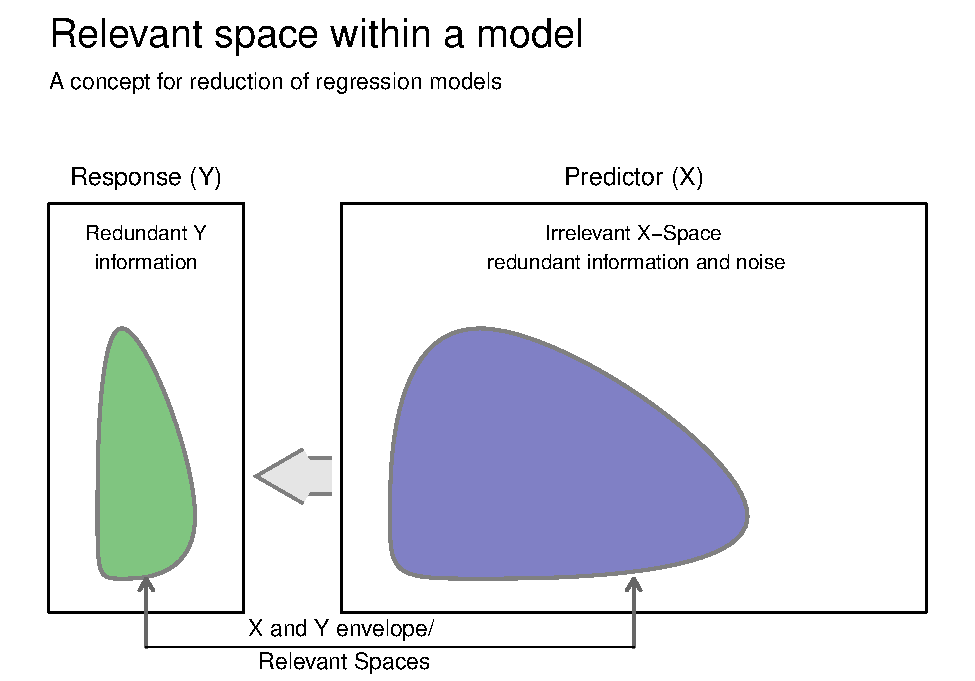
\includegraphics[width=0.8\linewidth]{Estimation-Paper_files/figure-latex/relevant-space-1} 

}

\caption{Relevant space in a regression model}\label{fig:relevant-space}
\end{figure}

Following the concept of relevant space, a subset of predictor
components can be imagined to span the predictor space. These components
can be regarded as relevant predictor components. \citet{Naes1985}
introduced the concept of relevant components which was explored further
by \citet{helland1990partial}, \citet{naes1993relevant},
\citet{Helland1994b} and \citet{Helland2000}. The corresponding
eigenvectors were referred to as relevant eigenvectors. A similar logic
is introduced by \citet{cook2010envelope} and later by
\citet{cook2013envelopes} as an envelope which is the space spanned by
the relevant eigenvectors \citep[, p.101]{cook2018envelope}. See
\citet{Rimal2018}, \citet{saebo2015simrel} and \citet{rimal2019pred} for
in-depth background on the model.

\section{Estimation Methods}\label{estimation-methods}

Let us departure from the linear model \eqref{eq:reg-model},

\begin{equation}
\underset{(1\times m)}{\mathbf{y}} =
  \underset{(1\times p)(p\times m)}
    {\mathbf{x}\boldsymbol{\beta}} +
  \underset{(1 \times m)}{\boldsymbol{\varepsilon}}
\label{eq:reg-model}
\end{equation}

where \(\mathbf{y}\) is a vector of \(m\) responses measured about their
means, \(\mathbf{x}\) is a vector of \(p\) predictors measured about
their means, \(\boldsymbol{\beta}\) is a matrix of regression
coefficients and \(\boldsymbol{\varepsilon}\) is a vector of independent
error terms with constant variance \(\boldsymbol{\Sigma}_{y|x}\). In
ordinary least squares, coefficient \(\boldsymbol{\beta}\) is estimated
as,

\begin{equation}
\underset{(p\times m)}{\boldsymbol{\hat{\beta}}} =
  \left(\underset{(p\times n)}{\mathbf{x}^t}
  \underset{(n\times p)}{\mathbf{x}}\right)^{-1}
  \underset{(p \times n)(n \times m)}{\mathbf{x}^t\mathbf{y}} =
  \mathbf{S}_{xx}^{-1}\mathbf{S}_{xy}
\label{eq:ols-coef}
\end{equation}

Let us define a transformation as \(\mathbf{z} = \mathbf{xR}\), where
\(\mathbf{R}\) is a \(p\times k\) matrix with orthogonal columns.
Regression model \eqref{eq:latent-model} defines a linear relationship of
these new variables \(\mathbf{z}\) with \(\mathbf{y}\) through the
coefficients \(\boldsymbol{\alpha}\).

\begin{equation}
\underset{(1 \times m)}{\mathbf{y}} =
  \underset{(1 \times k)}{\mathbf{z}}
    \underset{(k \times m)}{\boldsymbol{\alpha}} +
  \underset{(1 \times m)}{\boldsymbol{\varepsilon}}
\label{eq:latent-model}
\end{equation}

The coefficients \(\boldsymbol{\alpha}\) can be transformed back to
oritinal coefficients \(\boldsymbol{\beta}\) as
\(\boldsymbol{\beta} = \mathbf{R} \boldsymbol{\alpha}\). We can also
write a general form of regression coefficient \eqref{eq:ols-coef} as,

\[
\begin{aligned}
\underset{(p\times m)}{\boldsymbol{\hat{\beta}}} =
  \left[
    \underset{(p\times k)(k \times n)}{\mathbf{R}\mathbf{x}^t}
    \underset{(n\times k)(k \times p)}{\mathbf{x} \mathbf{R}^t}
  \right]^{-1}
  \underset{(p\times k)(k \times n)}{\mathbf{R}\mathbf{x}^t}
  \underset{(n\times m)}{\mathbf{y}} =
  \left[\mathbf{RS}_{xx}\mathbf{R}^t\right]^{-1}\mathbf{RS}_{xy}^t
\end{aligned}
\]

\emph{Principal Components Regression} (PCR) uses \(k\) eigenvectors of
\(\mathbf{S}_{xx}\) as the columns of \(\mathbf{R}\). Since PCR is based
on capturing the maximum variation in predictors on every components it
used to model, this method does not consider the response structure
\citep{Jolliffe2002}. In addition, if the relevant components are not in
the initial position, the method require more number of components to
make precise prediction \citep{rimal2019pred}.

\emph{Partial Least Squares} (PLS) regression on the other hand tries to
maximize the covariance between the predictors and the response scores
(SIMPLS paper). Broadly, PLS can be divided into PLS1 and PLS2 where the
former tries to model the response variables individually and the later
using all the response variable together while modeling. Among the three
widely used algorithms (NIPALS \citep{wold75nipals}, SIMPLS
\citep{DeJong1993} and KernelPLS \citep{Lindgren_1993}), for this study
we will be using KernelPLS which gires results equivalent to the rest
and is default in R-package \texttt{pls} \citep{mevik07_thepl}.

\emph{Envelopes} is first introduced by \citep{Cook2007a} as a smallest
subspace that include the span of regression coefficients.
\emph{Predictor Envelopes} (Xenv) identifies the envelope as a smallest
subspace in predictor space by separating the predictor covariance
\(\mathbf{S}_{xx}\) into relevant (material) and irrelevant (immaterial)
parts such that response \(\mathbf{y}\) is uncorrelated with the
irrelevant part given the relevant one. In addition, the relevant and
irrelevant parts are also uncorrelated. Such separation of the
covariance matrix is made using the data through optimization of
objective function. Further, the regression coefficients are estimated
only using the relevant part. \citet{cook2010envelope},
\citet{cook2013envelopes} and \citet{cook2018envelope} have extensively
discussed the foundation and various mathematical constructs together
with properties related to Predictor Envelope.

\emph{Simultaneous Predictor-Response Envelope} (Senv) implement the
envelope in both response and predictor spaces. It separates the
material and immaterial part in response space and predictor space such
that the material part of response does not correlate with the
immaterial part of predictor and the immaterial part of response does
not correlate with the material part of predictor. The regression
coefficients are computed using only the material part of the response
and predictor space. The number of components specified in both of these
methods during the fit influence the separation of these spaces. If the
number of response components is equals to the number of responses,
simultaneous envelope reduces to the predictor envelope and if the
number of predictor components is equals to the number of predictors,
the result will be equivalent to the ordinary least squares.
\citet{cook2015simultaneous} and \citet{cook2018envelope} have discussed
the method in detail. Further, \citet{helland2016algorithms} have
discussed how the population model of PCR, PLS and Xenv are equivalent.

\hypertarget{experimental-design}{\section{Experimental
Design}\label{experimental-design}}

An R \citep{coreR2018} package \texttt{simrel}
\citep{Rimal2018, saebo2015simrel} is used to simulate the data for
comparison. In the simulation the number of observation is fixed at
\(n = 100\) and following four simulation parameters are used to obtain
the data with wide range of properties.

\begin{description}
\tightlist
\item[\textbf{Number of predictors:}]
In order to cover both tall \((n>p)\) and wide \((p>n)\) cases,
\(p= 20\) and \(p= 250\) number of predictors are simulated.
\item[\textbf{Multicollinearity in predictor variables:}]
A parameter \texttt{gamma} \((\gamma)\) in simulation controls the
exponential decline of eigenvalues \((\lambda_i, i = 1, \ldots p)\)
corresponding to predictor variables as,

\begin{equation}
  \lambda_i = e^{-\gamma(i-1)}, \gamma > 0 \text{ and } i = 1, 2, \ldots p
  \label{eq:gamma}
  \end{equation}

Two levels 0.2 and 0.9 of \texttt{gamma} are used for simulation so that
level 0.2 simulates the data with low multicollinearity and 0.9
simulates the data with high multicollinearity.
\item[\textbf{Position of relevant components:}]
Initial principal components of a non-singular covariance matrix are
larger than the later one. If the principal components corresponding to
predictors with larger variation is not relevant for a response, this
will just increase noise in the data. Here we will use two different
levels of position index of predictor components: a) 1, 2, 3, 4 and b)
1, 2, 3, 4. Predictor components irrelevant for a response makes
prediction difficult \citep{Helland1994b}. When combined with
multicollinearity, this factor can create both easy and difficult model
for both estimation and prediction.
\item[\textbf{Correlation in response variables:}]
Many estimators also uses the structure of response for their
estimation. Here the correlation between the responses are varied
through a simulation parameter \texttt{eta} \((\eta)\). The parameter
controls the exponential decline of eigenvalues
\(\kappa_j, j = 1, \ldots m (\text{ number of responses})\)
corresponding to response variables as,

\begin{equation}
\eta_i = e^{-\kappa(j-1)}, \kappa > 0 \text{ and } j = 1, 2, \ldots m
\label{eq:eta}
\end{equation}

Four levels 0, 0.4, 0.8 and 1.2 of \texttt{eta} are used in the so that
level 0 simulates the data with uncorrelated response variables while
1.2 simulates the highly correlated response variables.
\end{description}

\begin{figure}
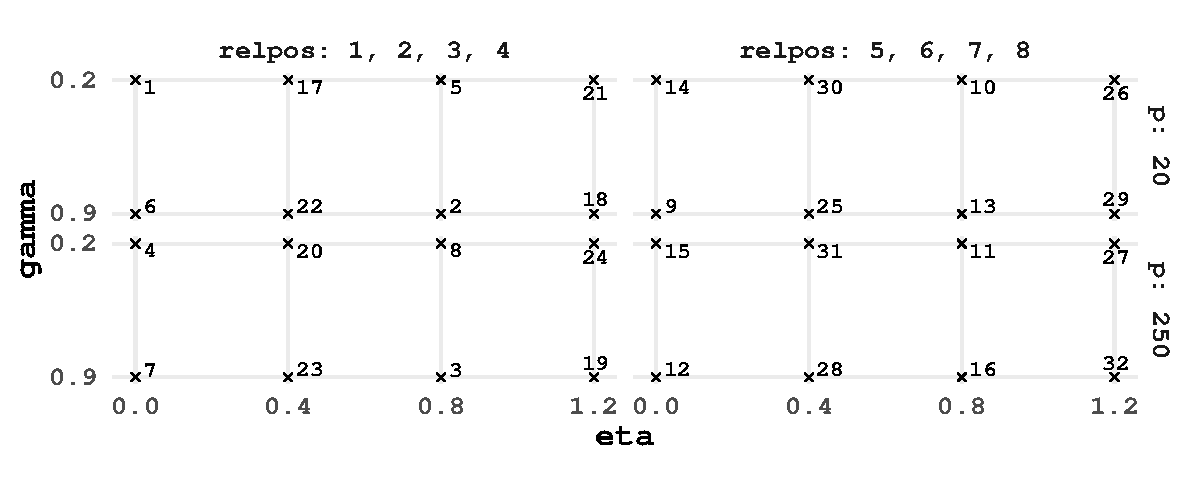
\includegraphics[width=1\linewidth]{Estimation-Paper_files/figure-latex/design-plot-1} \caption{Experimental Design of simulation parameters. Each point represents an unique data property.}\label{fig:design-plot}
\end{figure}

Here we have assumed that there is only one informative response
component. In the final dataset, all predictors together span the same
space as the relevant predictor components and all response together
span the same space as the one informative response component. In
addition, coefficient of determination is fixed at 0.8 for all dataset.

A complete factorial design is adopted using different levels of factors
discussed above to create 32 design (Figure \ref{fig:design-plot}) each
of which gives dataset with unique properties. From each of these design
and each estimation method, 50 different datasets are simulated so that
each of them have same true population structure. In total,
\(5 \times 32 \times 50\) i.e., 8000 datasets are simulated.






\begin{figure}
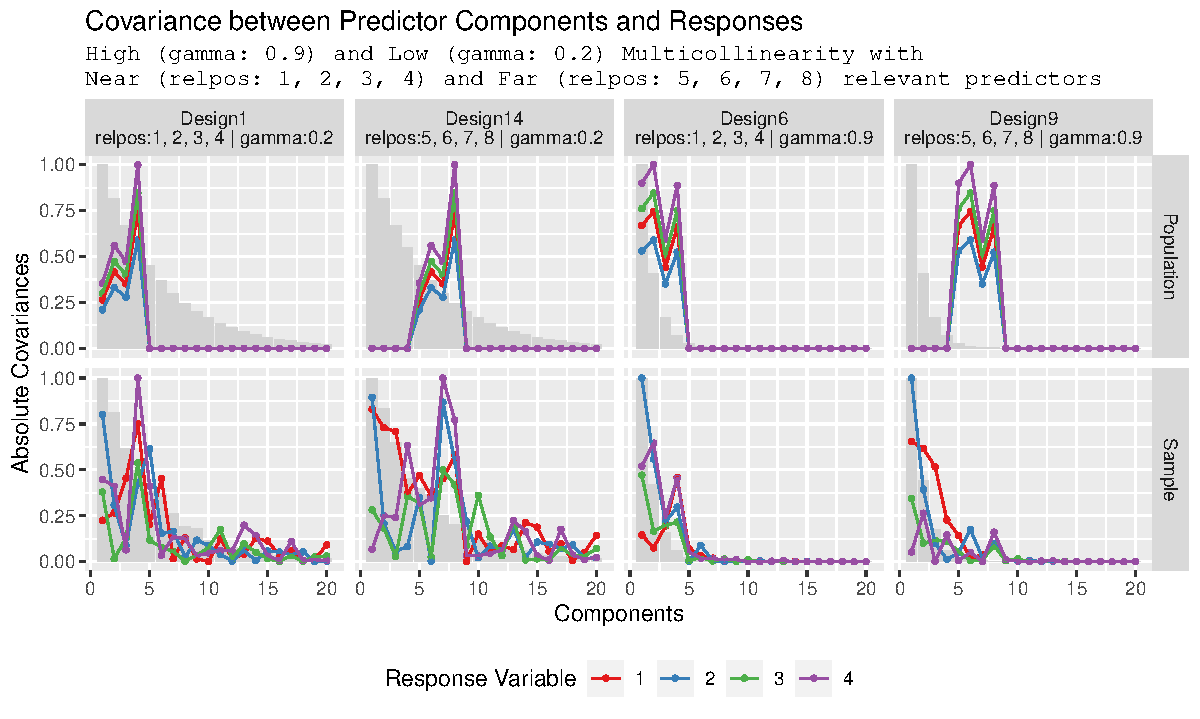
\includegraphics[width=1\linewidth]{Estimation-Paper_files/figure-latex/cov-plot-1} \caption{Covariance between predictor components and response
variables in population (top) and in the simulated data (bottom) for
four different designs. The Bar in the background represents the
variance of corresponding components.}\label{fig:cov-plot}
\end{figure}

The simulation properties are directly reflected in the simulated data.
For example, in Figure \ref{fig:cov-plot}, design pairs 1 and 4 as well
as 6 and 9 differs their properties only in terms of relevant predictor
components while the design pairs 1 and 6 as well as 14 and 9 differs
only in-terms of level of multicollinearity. The properties in
population are also reflected in the simulated samples.

\section{Basis of Comparison}\label{basis-of-comparison}

The focus of this study is to extend the exploration of
\citet{rimal2019pred} to compare the estimative performance of PCR,
PLS1, PLS2, Xenv and Senv methods. The performance is measured on the
basis of,

\begin{enumerate}
\def\labelenumi{\alph{enumi})}
\tightlist
\item
  average estimation error of the method using arbitrary number of
  components
\item
  average number of components used by the methods to give minimum
  estimation error
\end{enumerate}

Let us define the expected estimation error as,

\begin{equation}
\mathcal{EE}_{ijkl} =
  \mathsf{E}{\left[\left(\boldsymbol{\beta}_{ij} -
  \boldsymbol{\hat{\beta}_{ijkl}}\right)^t
  \left(\boldsymbol{\beta}_{ij} - \boldsymbol{\hat{\beta}_{ijkl}}\right)\right]}
\label{eq:est-error}
\end{equation}

for response \(j = 1, \ldots 4\) in a given design \(i=1, 2, \ldots 32\)
and method \(k=1(PCR), \ldots 5(Senv)\) using \(l=0, \ldots 10\) number
of components. Since both the expectation and the variance of
\(\hat{\boldsymbol{\beta}}\) are unknown, the prediction error are
estimated using data from 50 replications as follows,

\begin{equation}
\widehat{\mathcal{EE}_{ijkl}} =
  \frac{1}{50}\sum_{r=1}^{50}{\left[
  \left(\mathcal{EE}_\circ\right)_{ijklr}
  \right]}
\label{eq:estimated-est-error}
\end{equation}

where, \(\widehat{\mathcal{EE}_{ijkl}}\) is the estimated prediction
error averaged over \(r=50\) replicates and,
\[\left(\mathcal{EE}_\circ\right)_{ijklr} = \left(\boldsymbol{\beta}_{ij} -\boldsymbol{\hat{\beta}_{ijklr}}\right)^t\left(\boldsymbol{\beta}_{ij} - \boldsymbol{\hat{\beta}_{ijklr}}\right)\]

Our further discussion revolves around \emph{Error Dataset} and
\emph{Component Dataset} as in the prediction comparison paper
\citet{rimal2019pred}. For a given estimation method, design, and
response, the component that gives the minimum of estimation error
averaged over all replicates is selected as,

\begin{equation}
  l_\circ = \operatorname*{argmin}_{l}\left[\frac{1}{50}\sum_{r=1}^{50}{\left(\widehat{\mathcal{EE}}_\circ\right)_{r}}\right]
  \label{eq:min-err}
\end{equation}

The estimation error \(\widehat{\mathcal{EE}}_\circ\) for every methods,
design and response corresponding to \(l_\circ\) component, computed as
\eqref{eq:min-err}, is then regarded as \emph{error dataset} in the
subsequent analysis. Let \(\mathbf{u}_{8000\times4}=(u_j)\) for
\(j = 1, \ldots 4\) be the outcome variables measuring the estimation
error corresponding to the response \(j\) in the context of this
dataset. Further, let the number of components that result in minimum
estimation error in each replication be \(l_\circ\) computed as
\eqref{eq:min-comp} will be considred as \emph{component dataset}.

\begin{equation}
  l_{\circ} = \operatorname*{argmin}_{l}\left[\widehat{\mathcal{EE}}_{\circ}\right]
  \label{eq:min-comp}
\end{equation}

\hypertarget{exploration}{\section{Exploration}\label{exploration}}

This section explores the variation in the \emph{error dataset} and the
\emph{component dataset} for which we have used Principal Component
Analysis (PCA). Let \(t_u\) and \(t_v\) be the principal component score
sets corresponding to PCA run on the \(\mathbf{u}\) and \(\mathbf{v}\)
matrices respectively. The scores density in Figure
\ref{fig:est-pca-hist-mthd-gamma-relpos} and Figure
\ref{fig:comp-pca-hist-mthd-gamma-relpos} correspond to the first
principal component of \(\mathbf{u}\) and \(\mathbf{v}\), i.e.~the first
column of \(t_u\) and \(t_v\) respectively.





\begin{figure}[!htb]
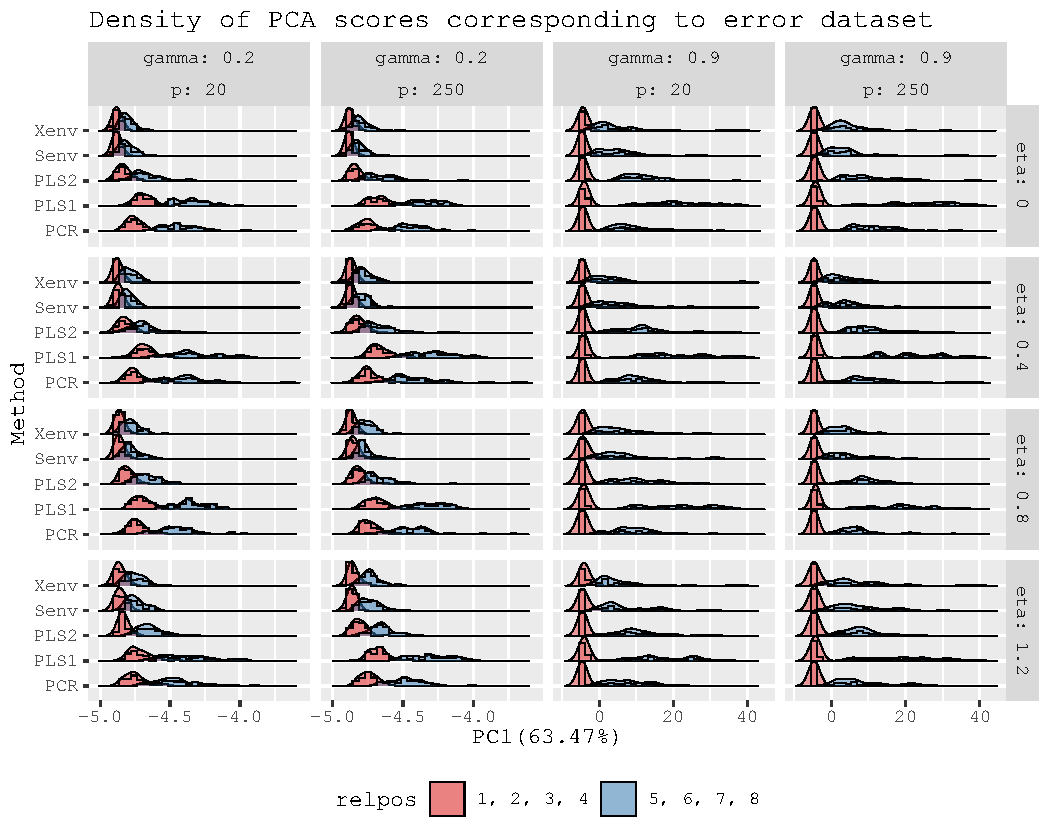
\includegraphics[width=1\linewidth]{Estimation-Paper_files/figure-latex/est-pca-hist-mthd-gamma-relpos-1} \caption{Scores density corresponding to first principal component
of \emph{error dataset} (\(\mathbf{u}\)) subdivided by \texttt{methods},
\texttt{gamma} and \texttt{eta} and grouped by \texttt{relpos}.}\label{fig:est-pca-hist-mthd-gamma-relpos}
\end{figure}

The plot shows a clear difference between the effect of low and high
multicollinearity in estimation error. In the case of low
multicollinearity (\texttt{gamma:\ 0.2}), the estimation errors are
smaller and have lesser variation compared to high multicollinearity
(\texttt{gamma:\ 0.9}). High multicollinearity has a larger influence on
all but noticeably in the methods based on envelopes. Some large
estimation error in the envelope is more than 100 which in the case of
other methods is less than 60.

Furthermore, the relevant predictor components, in general, has a
noticeable effect on estimation error. When relevant predictors are at
position 5, 6, 7, 8, the predictor components at 1, 2, 3, 4, which carry
most of the variation, becomes irrelevant. These irrelevant components
with large variation add noise to the model and consequently increases
the estimation error. The effect intensifies on highly collinear
predictors. Designs with high multicollinearity and relevant predictors
at position 5, 6, 7, 8 are relatively difficult to model for all the
methods. Although these difficult designs have a large effect on
estimation error, their effect on prediction error is less influential
\citep{rimal2019pred}.






In the case of the \emph{component dataset} (Figure Above), PCR, PLS1
and PLS2 methods have used more components in the case of high
multicollinearity compared to low. Surprisingly, the envelope methods
(Senv and Xenv) mostly have used a distinctly lesser number of
components in both the cases of multicollinearity compared to other
methods.

The plot also shows that there is no clear effect due to the correlation
of response variable on the number of components used to obtain minimum
estimation error.

\begin{figure}[!htb]
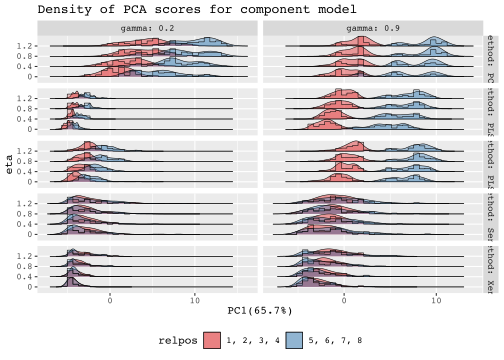
\includegraphics[width=1\linewidth]{Estimation-Paper_files/figure-latex/comp-pca-hist-mthd-gamma-relpos-1} \caption{Score density corresponding to first principal component
of \emph{component dataset} (\(\mathbf{v}\)) subdivided by
\texttt{methods}, \texttt{gamma} and \texttt{eta} and grouped by
\texttt{relpos}.}\label{fig:comp-pca-hist-mthd-gamma-relpos}
\end{figure}

A clear interaction between the position of relevant predictors and the
multicollinearity visible in the plot suggest that the methods use a
larger number of components when the relevant components are at position
5, 6, 7, 8. Additionally, the use of components escalate and the
difference between the two levels of \texttt{relpos} becomes wider in
the case of high multicollinearity in the model. Such performance is
also seen the the case of prediction error (See \citet{rimal2019pred})
however the number of components used in that case is lesser than in
this case. Envelope methods, however, have shown a distinct result in
contrast to the other methods. Even when the relevant predictors are at
position 5, 6, 7, 8, the envelope methods, in contrast to other methods,
have used an almost similar number of components as in the case of
relevant predictor at position 1, 2, 3, 4. This shows that the envelope
methods identify the predictor space relevant to the response
differently and with few numbers of latent components.

Following section explore the prediction and estimation error together
with the regression coefficient of Simultaneous Envelope and Partial
Least Squares for a design having high multicollinearity with predictor
components at position 5, 6, 7, 8. Here we will use design with \(n>p\)
and no correlation between the response which corresponds to Design-9.

\begin{figure}
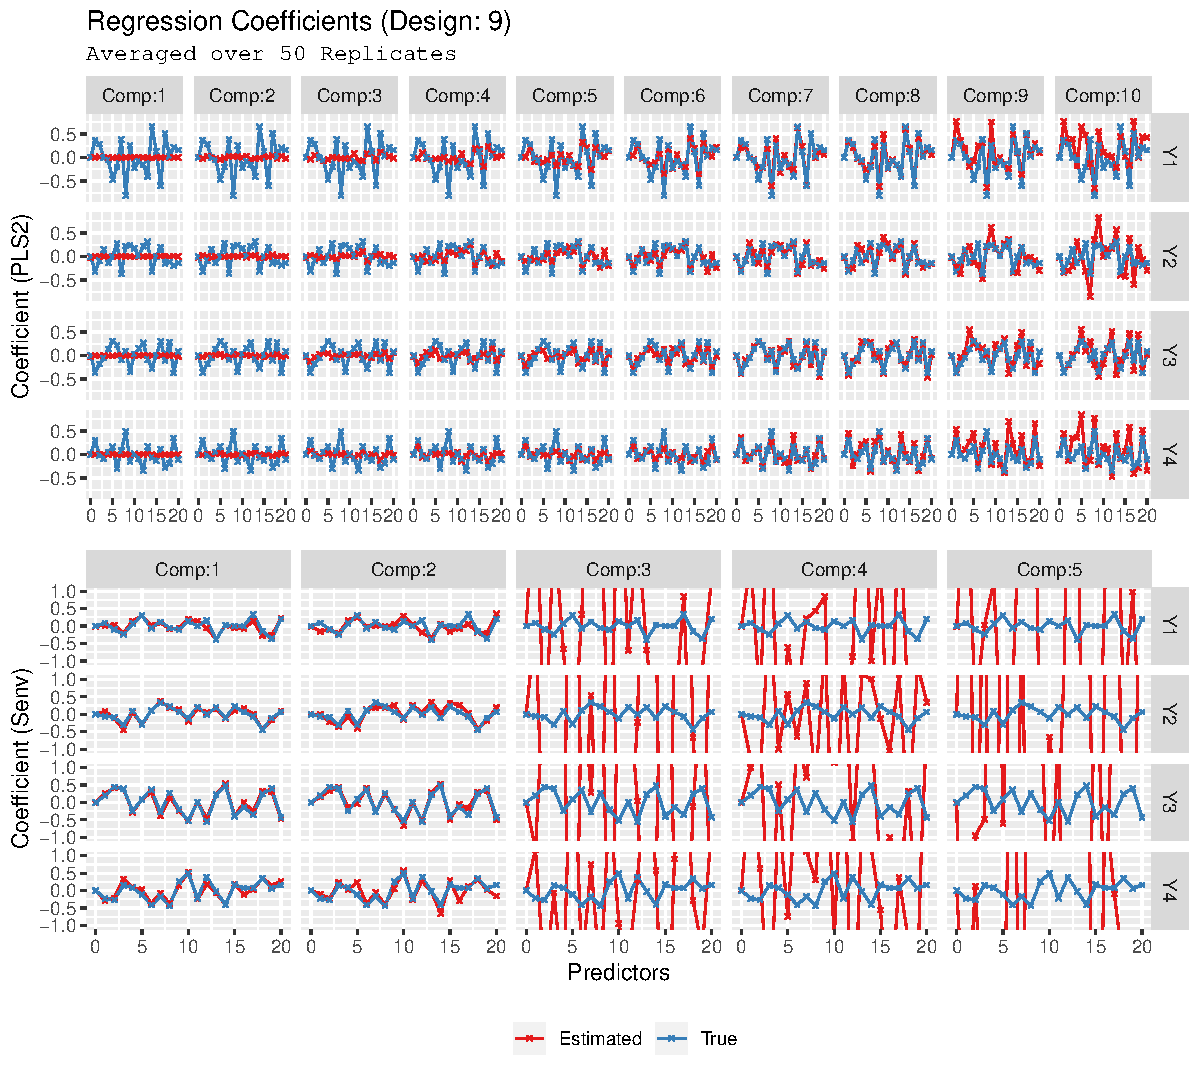
\includegraphics[width=1\linewidth]{Estimation-Paper_files/figure-latex/coef-plot-1} \caption{Regression Coefficients estimated by PLS2 and Simultaneous methods on the data based on Design 9.}\label{fig:coef-plot}
\end{figure}

Figure \ref{fig:err-plot} shows a clear distinction between the
modelling approach of PLS2 and Senv methods for the same model based on
Design 9. In the case of PLS2, both minimum prediction error and minimum
estimation error are obtained using seven to eight components and the
estimated regression coefficients approximate the true coefficients. In
contrast, the Senv method has approached the minimum prediction and
minimum estimation error using one to two components and the
corresponding estimated regression coefficients approximate the true
coefficients (Figure \ref{fig:coef-plot}). Despite having contrast
modelling result for a dataset with similar properties, the minimum
errors produced by them are comparable (See Table
\ref{tab:min-err-dgn9}).

\begin{figure}
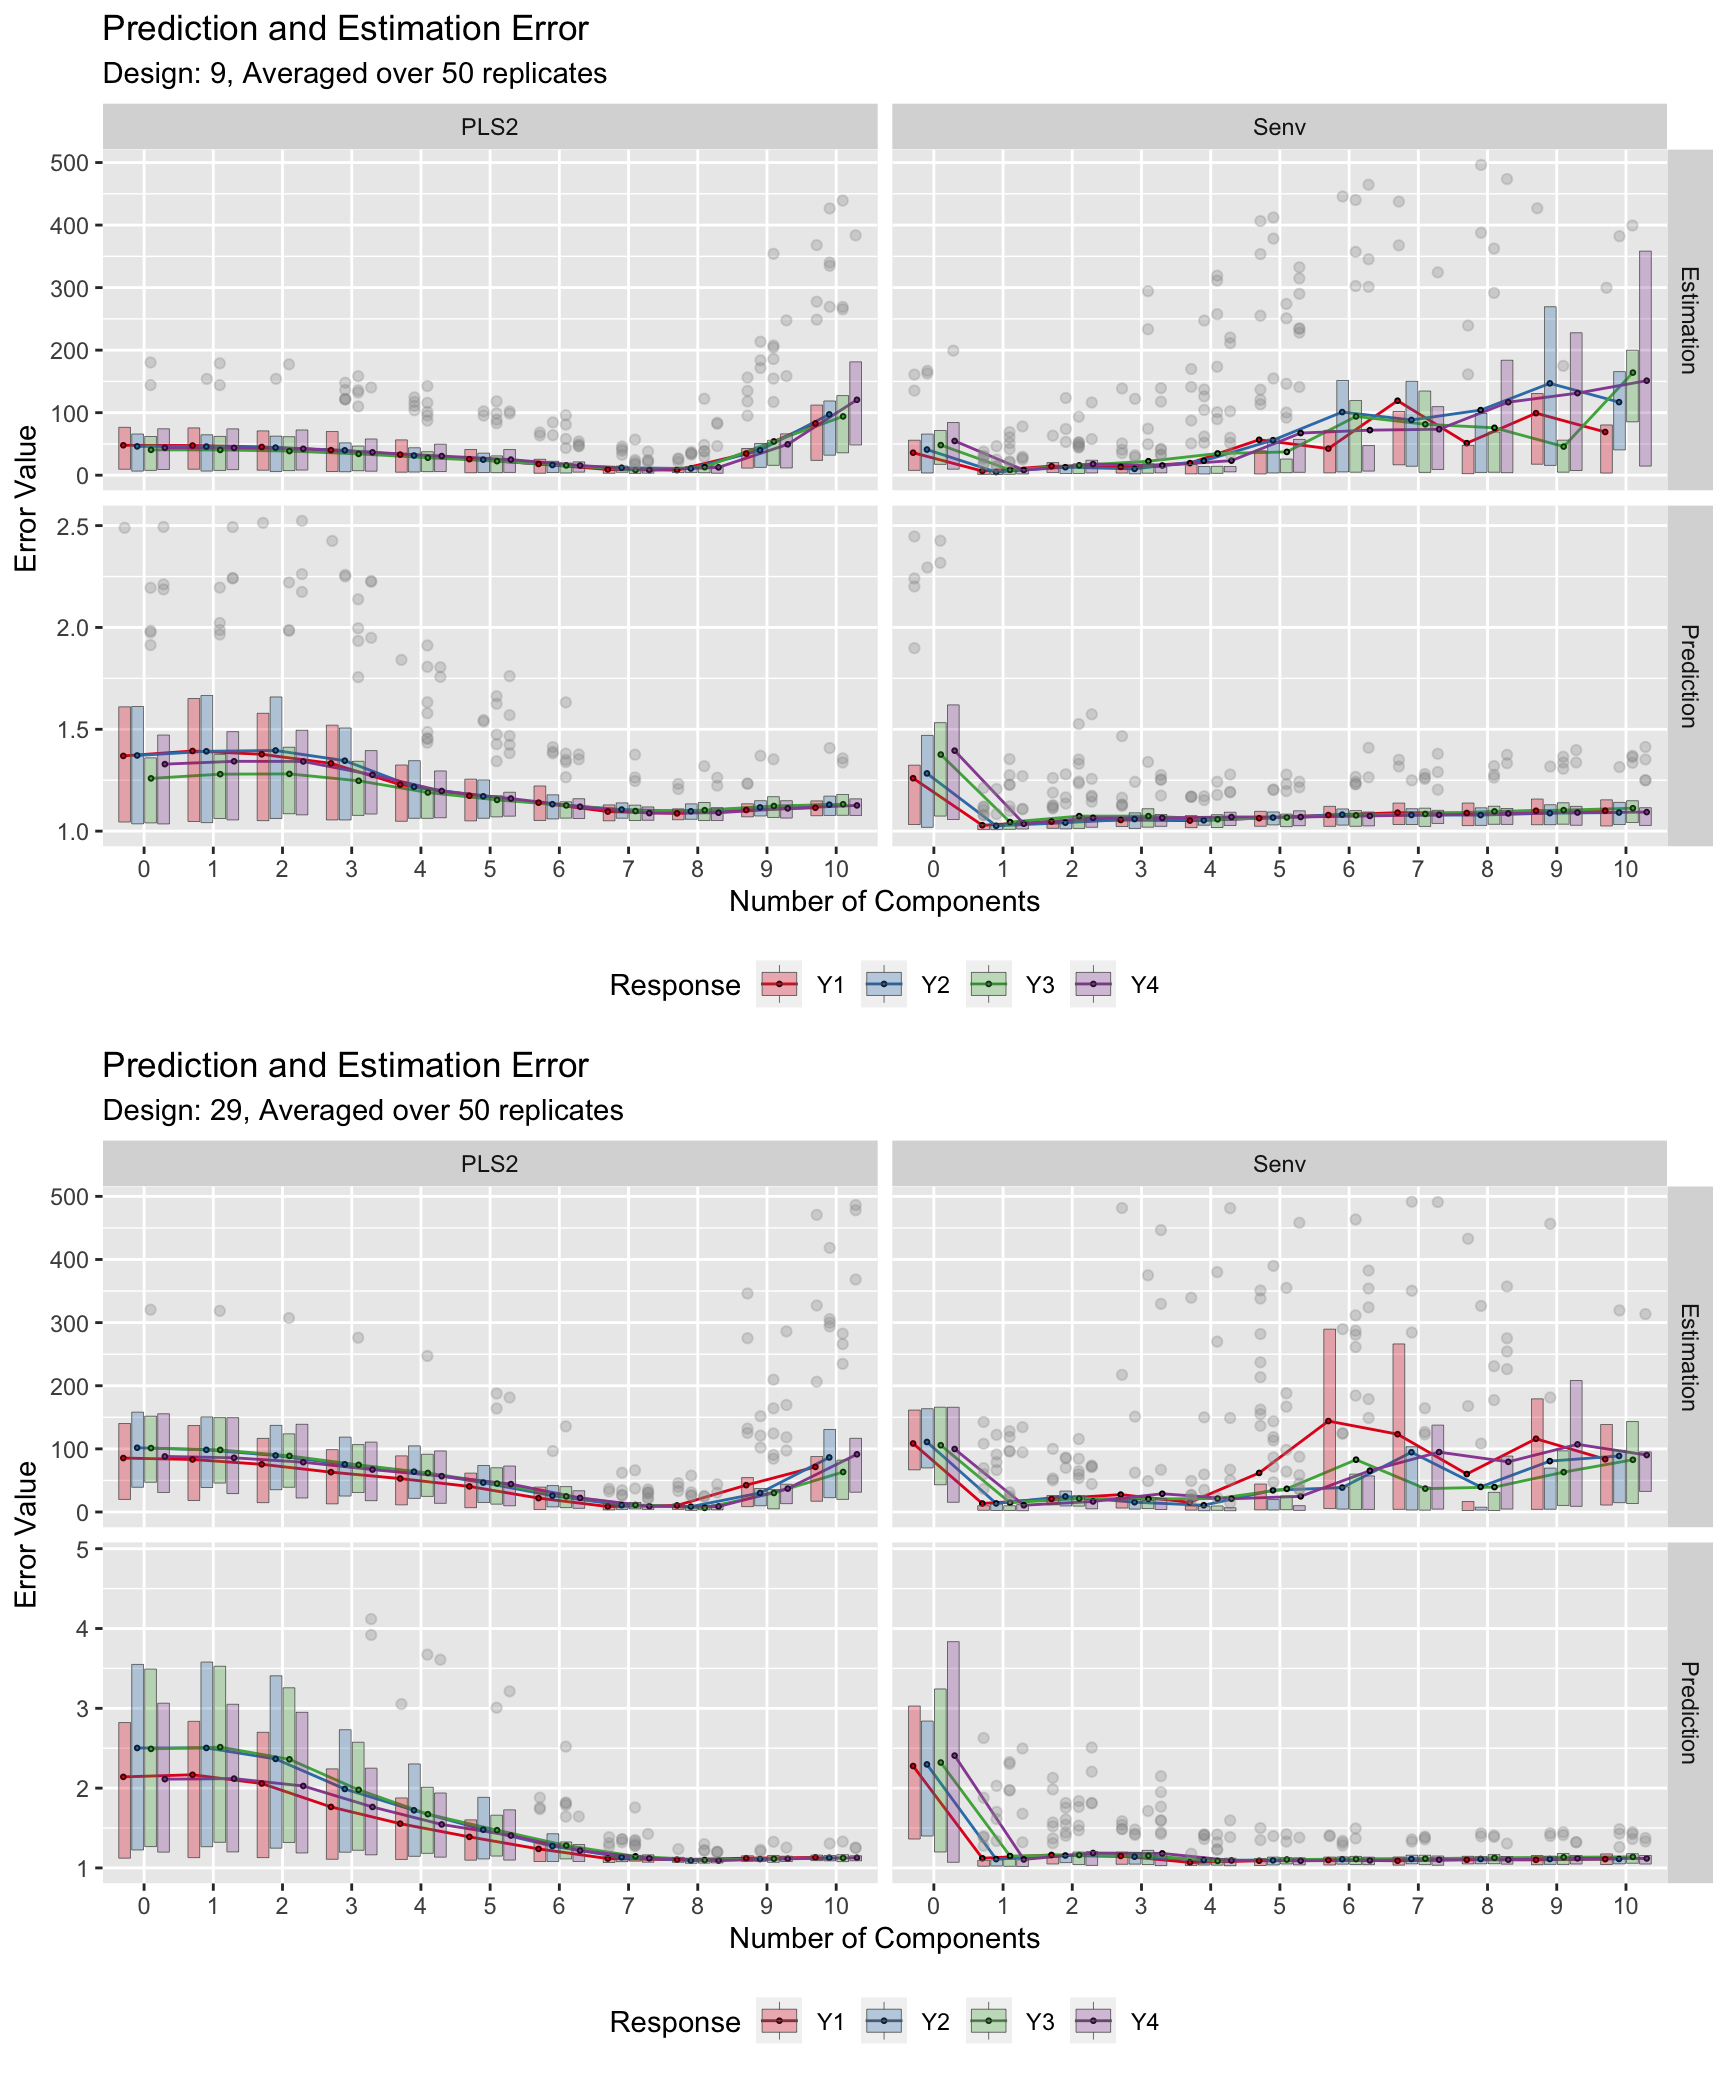
\includegraphics[width=1\linewidth]{Estimation-Paper_files/figure-latex/err-plot-1} \caption{Minimum prediction and estimation error for PLS2 and Simultaneous methods. The point and lines are averaged over 50 replications.}\label{fig:err-plot}
\end{figure}

The Figure \ref{fig:err-plot} also shows that Senv has resulted in huge
estimation error when the number of components is not optimal. This is
also true for the PLS2 model however the extent of this variation is
noticeably large in the Senv method. A similar observation as Senv is
also found in Xenv method while PCR and PLS1 are closer to the PLS2 in
terms of their use of components in order to produce the minimum error
(See Table \ref{tab:min-err-dgn9}).

\begin{verbatim}
List of 10
 $ name      : chr "kePrint"
 $ version   : chr "0.0.1"
 $ src       :List of 1
  ..$ file: chr "/usr/local/lib/R/site-library/kableExtra/kePrint-0.0.1"
 $ meta      : NULL
 $ script    : chr "kePrint.js"
 $ stylesheet: NULL
 $ head      : NULL
 $ attachment: NULL
 $ package   : NULL
 $ all_files : logi TRUE
 - attr(*, "class")= chr "html_dependency"
\end{verbatim}

\begin{table}[t]

\caption{\label{tab:min-err-dgn9}Minimum Prediction and Estimation Error for Design 9}
\centering
\begin{tabu} to \linewidth {>{\raggedleft}X>{\raggedleft}X>{\raggedleft}X>{\em}r>{\em}r>{\raggedleft}X}
\toprule
Response & PCR & PLS1 & PLS2 & Senv & Xenv\\
\midrule
\addlinespace[0.3em]
\multicolumn{6}{l}{\textbf{Estimation Error}}\\
\hspace{1em}1 & 8.56 (8) & 13.23 (6) & 8.17 (8) & 6.65 (1) & 5.73 (1)\\
\hspace{1em}2 & 7.94 (8) & 14.42 (6) & 10.65 (8) & 5.06 (1) & 5.35 (1)\\
\hspace{1em}3 & 7.02 (8) & 15.9 (6) & 8.22 (7) & 8.55 (1) & 5 (1)\\
\hspace{1em}4 & 9.26 (8) & 13.14 (7) & 8.29 (7) & 8.19 (1) & 4.78 (1)\\
\addlinespace[0.3em]
\multicolumn{6}{l}{\textbf{Prediction Error}}\\
\hspace{1em}1 & 1.08 (8) & 1.1 (7) & 1.09 (8) & 1.03 (1) & 1.03 (1)\\
\hspace{1em}2 & 1.09 (8) & 1.11 (7) & 1.1 (8) & 1.03 (1) & 1.03 (1)\\
\hspace{1em}3 & 1.08 (8) & 1.1 (7) & 1.1 (7) & 1.04 (1) & 1.03 (1)\\
\hspace{1em}4 & 1.09 (8) & 1.1 (7) & 1.09 (7) & 1.04 (1) & 1.03 (1)\\
\bottomrule
\end{tabu}
\end{table}

Despite having a large variation in prediction and estimation error, the
envelope based methods have produced a better result even in the
difficult model as obtained from Design 9.

\section{Analysis}\label{analysis}

A statistical analysis using Multivariate Analysis of variance (MANOVA)
model is performed on \emph{error dataset} and \emph{component dataset}
in order to understand the association between data properties and the
estimation methods. Let the corresponding models be \emph{error model}
\eqref{eq:err-model} and \emph{component model} \eqref{eq:comp-model}. In
the model, we will consider the interaction of simulation parameters
(\texttt{p}, \texttt{gamma}, \texttt{eta}, and \texttt{relpos}) and
\texttt{Method} The model is fitted using corresponding \emph{error
dataset} (\(\mathbf{u}\)) and \emph{component dataset} (\(\mathbf{v}\)).

\textbf{Error Model:}

\begin{equation}
  \mathbf{u} = \boldsymbol{\mu} +
  (\texttt{p} + \texttt{gamma} + \texttt{eta} +
    \texttt{relpos} + \texttt{Methods})^3 +
    \boldsymbol{\varepsilon}
  \label{eq:err-model}
\end{equation}

\textbf{Component Model:}

\begin{equation}
  \mathbf{v} = \boldsymbol{\mu} +
  (\texttt{p} + \texttt{gamma} + \texttt{eta} +
    \texttt{relpos} + \texttt{Methods})^3 +
    \boldsymbol{\varepsilon}
  \label{eq:comp-model}
\end{equation}

where, \(\mathbf{u}\) corresponds to the estimation errors in
\emph{error dataset} and \(\mathbf{v}\) corresponds to the number of
components used by a method to obtain minimum estimation error in the
\emph{component dataset}.

To make the analysis equivalent to \citet{rimal2019pred}, we have also
used Pillai's trace statistic for accessing the result of MANOVA. Figure
\ref{fig:manova-plot} plots the Pillai's trace statistics as bars with
corresponding F-values as text labels. The left plot corresponds to the
\emph{error model} and the right plot corresponds to the \emph{component
model}.





\begin{figure}
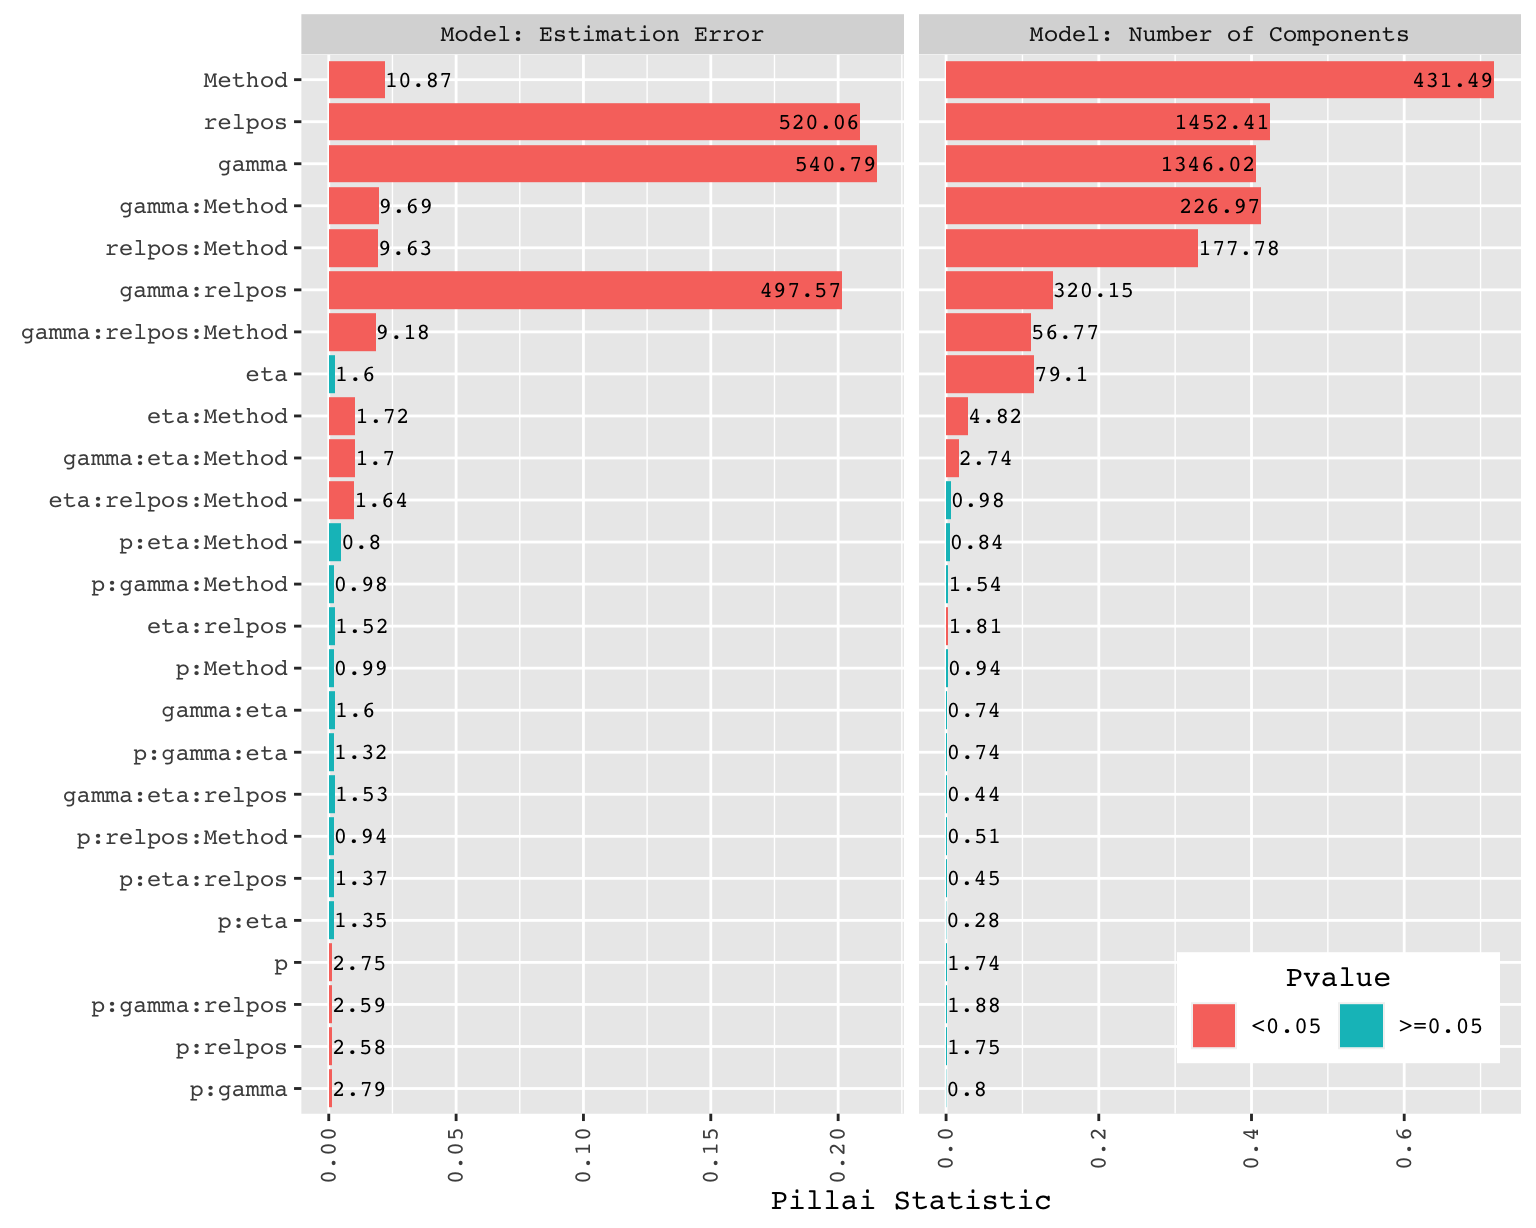
\includegraphics[width=1\linewidth]{Estimation-Paper_files/figure-latex/manova-plot-1} \caption{Pillai Statistic and F-value for the MANOVA model. The
bar represents the Pillai Statistic and the text labels are F-value for
corresponding factor.}\label{fig:manova-plot}
\end{figure}

\begin{description}
\tightlist
\item[\textbf{Error Model:}]
Unlike prediction error in \citet{rimal2019pred}, \texttt{Method} has a
lesser effect while the amount of multicollinearity controlled by
\texttt{gamma} parameter has a huge effect in the case of estimation
error (Figure \ref{fig:manova-plot}). In addition, the position of
relevant predictors and its interaction with the \texttt{gamma}
parameters also have a substantial effect on the estimation error. This
also supports the results seen in the
\protect\hyperlink{exploration}{Exploration} section where relevant
predictors at position 5, 6, 7, 8 with high multicollinearity design
creates large uninformative variance in the components 1, 2, 3, 4 making
the design difficult. The effect of this on the estimation error is much
larger than on the prediction error.

Furthermore, the \texttt{eta} factor controlling the correlation between
the responses, and its second-order interaction with other factors
except for the number of predictors is significant. The effect is also
comparable with the main effect of \texttt{Method} and \texttt{eta}.
\item[\textbf{Component Model:}]
Although the \texttt{Method} does not have a large impact on the
estimation error, the \emph{component model} in Figure
\ref{fig:manova-plot} (right) shows that the methods are significantly
different and has a huge effect on the number of components they use to
obtain the minimum estimation error. The result also corresponds to the
case of prediction error in \citet{rimal2019pred}. However, the F-value
corresponding the \texttt{relpos} and \texttt{gamma} shows that the
significance of these factors are much stronger compared to the case of
prediction error.
\end{description}

We will further explore the effects of individual levels of different
factors in the following subsection.

\subsection{Effect Analysis of the Error
Model}\label{effect-analysis-of-the-error-model}

In figure \ref{fig:est-eff-plots} (left), the effect of correlation
between the responses controlled by \texttt{eta} parameter has a clear
influence on the estimation error and the effect is highly dependent on
the estimation methods. In the case of envelope methods, the effect of
\texttt{eta} on estimation error is smaller than other methods and are
similar in the case of both levels of the position of relevant
predictors (\texttt{relpos}). However, PCR, PLS1 and PLS2 have shown a
clear difference in the estimation error for four different levels of
response correlation. The error in the case of relevant predictors at
position 5, 6, 7, 8 is huge as compared to the case where relevant
predictors are at position 1, 2, 3, 4. Among these methods, PLS1 has the
highest estimation error in both levels of relevant predictors since the
method models the response variables independently and does not consider
the correlation structure in them.




\begin{figure}
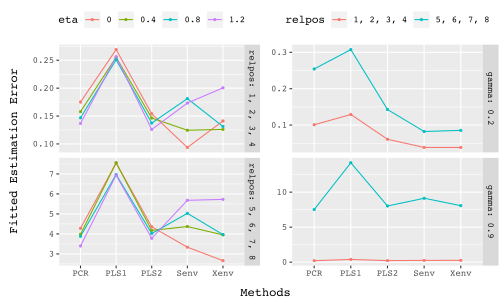
\includegraphics[width=1\linewidth]{Estimation-Paper_files/figure-latex/est-eff-plots-1} \caption{Effect plot of some interactions of the multivariate
linear model of estimation error}\label{fig:est-eff-plots}
\end{figure}

Figure \ref{fig:est-eff-plots} (right) shows the large difference in the
effect of two levels of the position of relevant predictors especially
in the designs with high multicollinearity. In the case of high
multicollinearity, all methods have noticeable poor performance compared
to the case of low multicollinearity.

Figure \ref{fig:est-eff-plots} also shows that PCR and PLS2 methods have
the smallest effect on the estimation error in both levels of relevant
predictors in the case of moderate to high level of correlation present
in the response. In the case of low correlation, envelope methods have
the smallest estimation error. Similarly, the designs with low
multicollinearity are favourable to the envelope methods. Their
estimation errors in these cases are smaller than other methods.

\subsection{Effect Analysis of the Component
Model}\label{effect-analysis-of-the-component-model}

In the case of \emph{component model}, envelope methods are the clear
winner in almost all designs. In the case of low multicollinearity and
position of relevant predictors at 1, 2, 3, 4, PLS1 has obtained the
minimum estimation error similar to the envelope methods, however in the
case of high multicollinearity PLS1 has also used a fairly large number
of components to obtain the minimum prediction error. It is interesting
to observe that the envelope methods have comparable and minimum
estimation error in most of the designs have used 1-2 components on
average. The effect of the correlation in the response has minimal
effect on the number of components used by the methods. The design nine
which we have considered in the previous section has minimum estimation
error from envelope methods using at most 2 components by Xenv and 3
components by Senv. This corresponds with the results seen in Figure
\ref{fig:comp-eff-plots}.




\begin{figure}[!htb]
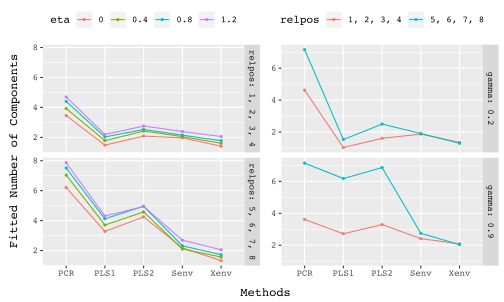
\includegraphics[width=1\linewidth]{Estimation-Paper_files/figure-latex/comp-eff-plots-1} \caption{Effect plot of some interactions of the multivariate
linear model of number of components to get minimum prediction error}\label{fig:comp-eff-plots}
\end{figure}

\section{Discussion and Conclusion}\label{discussion-and-conclusion}

\begin{itemize}
\tightlist
\item
  A similar discussion but based more on why the methods worked in the
  way we have seen in the results in previous sections
\item
  Some concluding remarks and limitations (or a gate for further
  exploration)
\end{itemize}

\hypertarget{refs}{}


\renewcommand\refname{References}
\bibliography{References.bib}


\end{document}
